\documentclass[a4paper]{article}

\usepackage[utf8]{inputenc}
\usepackage[T2A]{fontenc}
\usepackage[english, russian]{babel}
\usepackage[normalem]{ulem}
\usepackage{fancyhdr}
\usepackage{extramarks}
\usepackage{amsfonts}
\usepackage{amsmath}
\usepackage{amssymb}
\usepackage{amsthm}
\usepackage[colorlinks=true,draft=false, allcolors=blue]{hyperref}
\usepackage{dirtytalk}
\usepackage{xcolor}
\usepackage{multicol}
\usepackage[twoside=false,top=16mm,bottom=10mm,left=4mm,right=4mm]{geometry}
\usepackage{listings}
\usepackage{lastpage}

\pagestyle{fancy}
\lhead{\small{СУНЦ МГУ + ЦПМ: Сборная СОСквы (Понкратов, Пугачёв, Шатохин)}}
\rhead{\thepage/\pageref*{LastPage}}
\fancyheadoffset[L,R]{0pt}
\cfoot{}

\setlength{\parindent}{0.0in}

\lstset{
	tabsize=4,
    basicstyle=\ttfamily\scriptsize,
    columns=fullflexible,
    showstringspaces=false,
    extendedchars=true,
    breaklines=true,
    prebreak=\raisebox{0ex}[0ex][0ex]{},
    frame=single,
    showtabs=false,
    showspaces=false,
    keepspaces=true,
    keywordstyle=\bfseries\color{green!40!black},
    commentstyle=\itshape\color{purple!40!black},
    identifierstyle=\color{blue},
    stringstyle=\color{orange},
    % belowcaptionskip=1\baselineskip,
    % breaklines=true,
    % frame=single,
    % xleftmargin=\parindent, !
    % language=C++, !
    % showstringspaces=false,
    % basicstyle=\footnotesize\ttfamily,  
}

\begin{document}

\begin{multicols*}{2}
% \begin{multicols*}{3}

    \tableofcontents

    \section{Общее}
        \begin{itemize}
    \item Собственное вращение на угол $\varphi$ с центром вращения в начале координат: \\ $x' = x \cos \varphi - y \sin \varphi \\ 
    y' = x \sin \varphi + y \cos \varphi$
    \item Расстояние между точками по сфере: 
    $L = R \cdot \arccos(\cos \theta_{1} \cdot \cos \theta_{2} + \sin \theta_{1} \cdot \sin \theta_{2} \cdot \cos(\varphi_{1} - \varphi_{2}))$
    где $\theta$ – широты (от $-\pi$ до $\pi$), $\varphi$ – долготы (от $-\pi$ до $\pi$)
    \item Объем шарового сегмента: $V = \pi h^{2}(R - \frac{1}{3}h)$, где $h$ -- высота от вершины сектора до секущей плоскости
    \item Площадь поверхности шарового сегмента: $S = 2\pi Rh$, где $h$ -- высота
    % \item $2^{23} \cdot 7 \cdot 17 + 1 = 998.244.353$ --- простое, первообразный корень -- $3$
    \item Код Грея: $g_{n} = n \oplus \frac{n}{2}$
    \item Числа Фибоначчи: \\ $\displaystyle F_{0} = 0, F_{1} = 1, F_{n} = \frac{(\frac{1 + \sqrt{5}}{2})^{n} - (\frac{1 - \sqrt{5}}{2})^{n}}{\sqrt{5}}$
    \item Sum-xor property: $a + b = a \oplus b + 2(a\&b), a + b = a|b + a\&b, a \oplus b = a|b - a\&b$
    \item Число граней в планарном графе(с учётом бесконечной): $R = 2 - V + E$
    \item Сумма арифметической прогрессии: $S_{n} = \frac{n(a_{1} + a_{n})}{2}$
    \item Сумма геометрической прогрессии: $S_{n} = \frac{b_{1}(q^{n} - 1)}{q - 1}$
    \item Определители матриц
    $$
    \left|
    \begin{array}{c c}
        a & b \\
        c & d
    \end{array}
    \right| = ad - bc
    $$
    \begin{multline*}
    \left|
    \begin{array}{c c c}
        a_{1} & b_{1} & c_{1} \\
        a_{2} & b_{2} & c_{2} \\
        a_{3} & b_{3} & c_{3} \\
    \end{array}
    \right| = a_{1}b_{1}c_{1} + a_{3}b_{1}c_{2} + a_{2}b_{3}c_{1} -\\- a_{3}b_{2}c_{1} - a_{1}b_{3}c_{2} - a_{2}b_{1}c_{3}
    \end{multline*}
    $\Delta = \sum_{j = 1}^{n} (-1)^{j + 1} \cdot a_{1, j} \cdot \bar{M_{j}^{1}}$, $\bar{M_{j}^{1}}$ --- определитель матрицы, полученной вычеркиванием $1$ строки и $j$ стоблца.
    \item \textbf{Метод Крамера.} $\det A \neq 0 \implies$ единственное решение. Иначе $0$ или $\infty$.
    Решения: $\displaystyle x_{i} = \frac{\Delta_{i}}{\Delta}$. В $\Delta_{i}$ столбец коэффициентов при соответствующей неизвестной заменяется столбцом свободных членов системы.
\end{itemize}

    
    \section{Коды}
        
        \subsection{Basic setup}
            \lstinputlisting[language=C++]{src/basic_setup/template.cpp}

        \subsection{Бесполезное}
            Санитайзеры:
                \lstinputlisting[language=C++]{src/basic_setup/sanitize.txt}
            
            Прагмы:
                \lstinputlisting[language=C++]{src/basic_setup/pragmas.cpp}
            
            Встроенный декартач:
                \lstinputlisting[language=C++]{src/basic_setup/orderedset.cpp}
                
            Atomic hashset, hashmap:
                \lstinputlisting[language=C++]{src/basic_setup/hashmap.cpp}
                
            Перебор всех подмасок и надмасок:
                \lstinputlisting[language=C++]{src/basic_setup/masks.cpp}
    
        \subsection{Мосты}
            \lstinputlisting[language=C++]{src/graph/bridges.cpp}
            
        \subsection{Точки сочленения}
            \lstinputlisting[language=C++]{src/graph/cutpoints.cpp}
            
        \subsection{DCP (TheEvilBird)}
            \lstinputlisting[language=C++]{src/graph/dcp_theevilbird.cpp}
        
        \subsection{MaxFlow (TheEvilBird)}
            \lstinputlisting[language=C++]{src/graph/maxflow_theevilbird.cpp}
                
        \subsection{MinCostMaxFlow (TheEvilBird)}
            \lstinputlisting[language=C++]{src/graph/mincost_theevilbird.cpp}
        
        \subsection{Эйлеров цикл}
            \lstinputlisting[language=C++]{src/graph/euler.cpp}

        \subsection{Кун}
            \lstinputlisting[language=C++]{src/graph/kuhn.cpp}

        Вершинное покрытие графа --- множество вершин, что каждое ребро графа инцидентно хотя бы одной вершине из множества.
        
        Пусть $M$ --- макс. парсоч. Мысленно ориентируем ребра графа: ребра из $M$ проведем из правой доли в левую, остальные --- из левой в правую, 
        после чего запустим обход в глубину из всех вершин левой доли, не включенных в $M$.
        Граф разбился на несколько множеств: $L^{+}$, $L^{-}$, $R^{+}$, $R^{-}$, где <<плюсовые>> множества --- это множества посещенных в процессе обхода вершин. Тогда $V_{min} = L^{-} \cup R^{+}$.

        Независимое множество вершин ---  множество вершин, что никакая пара вершин не соединена ребром. Дополнение минимального вершинного покрытия является максимальным независимым множеством.

        Покрытие дага путями: $n - matching$
        
        \subsection{HLD (TheEvilBird)}
            \lstinputlisting[language=C++]{src/graph/hld_theevilbird.cpp}

        \subsection{Dominator tree (TheEvilBird)}
            \lstinputlisting[language=C++]{src/graph/dominator_teb.cpp}

        \subsection{Link-Cut (TheEvilBird)}
            \lstinputlisting[language=C++]{src/ds/linkcut_theevilbird.cpp}
        
        \subsection{Личао (FedShat)}
            \lstinputlisting[language=C++]{src/geom/lichao_fedshat.cpp}
            
        \subsection{Segment Tree (TheEvilBird)}
            \lstinputlisting[language=C++]{src/ds/segtree_theevilbird.cpp}
        
        \subsection{Segment Tree Down (TheEvilBird)}
            \lstinputlisting[language=C++]{src/ds/segtree_down_theevilbird.cpp}
        
        \subsection{Segment Tree Beats (TheEvilBird)}
            \lstinputlisting[language=C++]{src/ds/segtree_beats_theevilbird.cpp}
        
        \subsection{Persistent Segment Tree (Sweezyk)}
            \lstinputlisting[language=C++]{src/ds/pers_segtree_sweezyk.cpp}
            
        \subsection{Fenwick (TheEvilBird)}
            \lstinputlisting[language=C++]{src/ds/fenwick_theevilbird.cpp}
        
        \subsection{Sparse table (TheEvilBird)}
            \lstinputlisting[language=C++]{src/ds/sparse_theevilbird.cpp}
        
        \subsection{Treap (Sweezyk)}
            \lstinputlisting[language=C++]{src/ds/treap_sweezyk.cpp}
        
        \subsection{Extended GCD (Sweezyk)}
            \lstinputlisting[language=C++]{src/math/ext_gcd_sweezyk.cpp}
        
        \subsection{FFT (FedShat)}
            \lstinputlisting[language=C++]{src/math/fft_fedshat.cpp}
        
        \subsection{КТО (FedShat)}
            \lstinputlisting[language=C++]{src/math/kto_fedshat.cpp}
        
        \subsection{Обратные по простому модулю}
            Пусть дан простой модуль $m$. Для каждого числа из $[1, m - 1]$ найти обратное к нему.
            \lstinputlisting[language=C++]{src/math/rev_from_1_to_mod.cpp}
        
        \subsection{Обратные факториалы}
            \lstinputlisting[language=C++]{src/math/rev_fact.cpp}
        
        \subsection{Гаусс}
            \lstinputlisting[language=C++]{src/math/gauss.cpp}
            
            \textbf{Бинарный}
            \lstinputlisting[language=C++]{src/math/bin_gauss.cpp}
        
        \subsection{Быстрая факторизация (FedShat)}
            \lstinputlisting[language=C++]{src/math/fact_fedshat.cpp}

        \subsection{Префикс-функция}
            \lstinputlisting[language=C++]{src/string/prefix_func.cpp}
            
        \subsection{Z-функция}
            \lstinputlisting[language=C++]{src/string/z_func.cpp}
            
        \subsection{Суфмас (TheEvilBird)}
            \lstinputlisting[language=C++]{src/string/sufarray_theevilbird.cpp}
            
        \subsection{Суфавтомат (TheEvilBird)}
            \lstinputlisting[language=C++]{src/string/sufavtomat_theevilbird.cpp}
        
        \subsection{Ахо-Корасик (Sweezyk)}
            \lstinputlisting[language=C++]{src/string/korasik_sweezyk.cpp}
            
        \subsection{Манакер}
            \lstinputlisting[language=C++]{src/string/manacher.cpp}
            
        \subsection{CHT (FedShat)}
            \lstinputlisting[language=C++]{src/geom/cht_fedshat.cpp}
        
        \subsection{Дебаг Туриста}
            \lstinputlisting[language=C++]{src/basic_setup/debug.cpp}
        
        % \newpage
        \subsection{Геометрия (TheEvilBird)}
            \lstinputlisting[language=C++]{src/geom/geom_theevilbird.cpp}

        \subsection{Стрессы (TheEvilBird)}
            \lstinputlisting[language=Python]{src/stress/generators.py}
    
\end{multicols*}

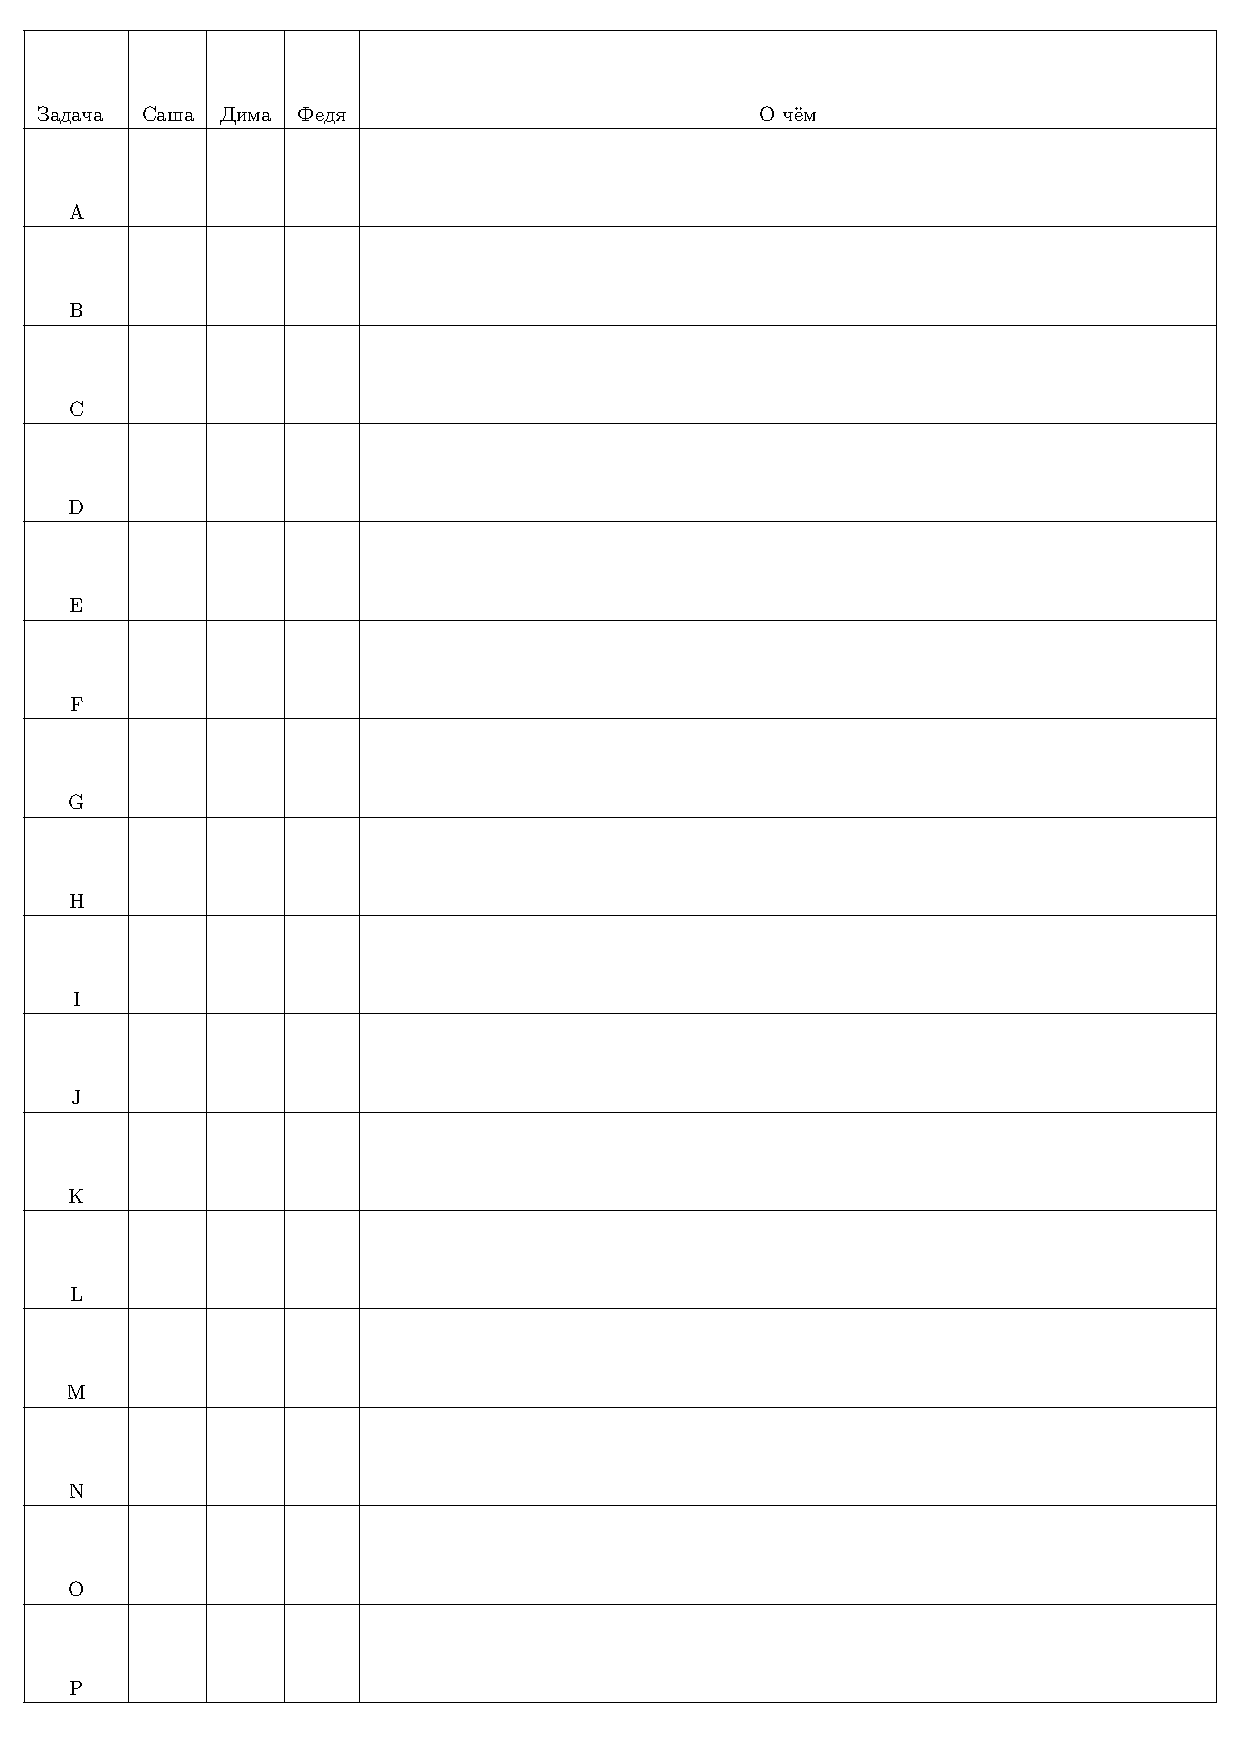
\includepdf{src/table.pdf}

\end{document}

